\originalchapter{作业六至十：传播与光学}
本章依据 MIT 8.03SC Fall 2016 的 Homework 6--10 整理中文题面. 原件只提供题目, 下列解答为 AI 独立推导, 不是 MIT 官方解答. 图示由原图核对后以文字或 TikZ 重绘; 读图量保留近似性质.

\originalsection{作业六}
\begin{exercise}\label{ps:6.1}
原题 Problem 6.1 (25 pts). 风琴管中空气体积元的纵向位移 $\psi$ 满足 $\psi_{tt}=A\psi_{xx}$, $A=90000\,\mathrm{m^2/s^2}$. 管在 $x=0$ 封闭, 在 $x=L=1.5\,\mathrm m$ 开口.
\begin{enumerate}[label=\alph*.]
\item 在 $0\le x\le L$ 画前三个简正模的最大位移形状, 写出各自频率. 只需边界条件的物理理解和简单计算.
\item 画前三个模的最大压力振幅随 $x$ 的形状.
\item 改为两端开口时, 为保留基频, 管应多长?
\end{enumerate}
\end{exercise}
\begin{solution}
声速 $v=\sqrt A=300\,\mathrm{m/s}$. 封闭端是位移节点, 开口端是压力节点, 即 $\psi(0)=0$, $\psi_x(L)=0$. 因而
\[
 k_n=\frac{(2n-1)\pi}{2L},\quad \psi_n(x,t)=D_n\sin(k_nx)\cos(\omega_nt),\quad
 f_n=\frac{(2n-1)v}{4L}.
\]
(a) 前三频率为 $50,150,250\,\mathrm{Hz}$. (b) 若空气体积模量为 $K$, 压强扰动 $p'=-K\psi_x$, 空间形状为 $-\cos(k_nx)$, 封闭端压力腹、开口端压力节点. 图中每条曲线分别归一; 实线是位移, 虚线是压强, 正负整体可倒转.
\begin{center}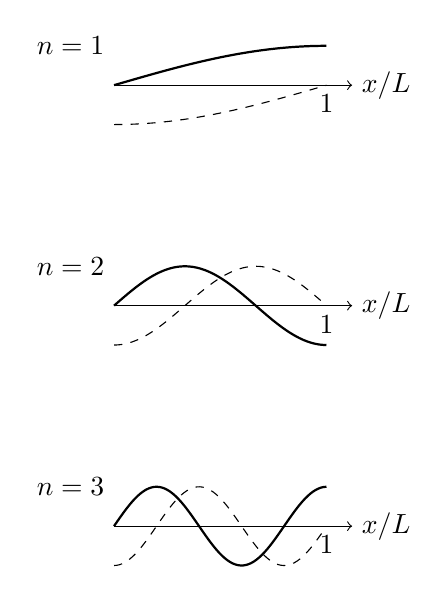
\begin{tikzpicture}[x=2.7cm,y=.5cm]
\foreach \n in {1,2,3}{
\begin{scope}[yshift={-2.8*\n cm}]
\draw[->] (0,0)--(1.12,0) node[right]{$x/L$};
\draw[thick,domain=0:1,samples=80] plot (\x,{sin((2*\n-1)*90*\x)});
\draw[dashed,domain=0:1,samples=80] plot (\x,{-cos((2*\n-1)*90*\x)});
\node[left] at (0,1){$n=\n$};\node[below] at (1,0){$1$};
\end{scope}}
\end{tikzpicture}\end{center}
(c) 两端开口基频为 $v/(2L')$, 等于原基频 $v/(4L)$, 故 $L'=2L=3.0\,\mathrm m$.
\end{solution}

\begin{exercise}\label{ps:6.2}
原题 Problem 6.2 (25 pts). 课堂由 Maxwell 方程讨论了电磁波, 但未完成磁场波动方程的推导.
\begin{enumerate}[label=\alph*.]
\item 对向量场 $\mathbf A$ 证明 $\nabla\times(\nabla\times\mathbf A)=\nabla(\nabla\cdot\mathbf A)-\nabla^2\mathbf A$.
\item 用真空 Maxwell 方程证明 $\nabla^2\mathbf B=\mu_0\epsilon_0\mathbf B_{tt}$.
\end{enumerate}
\end{exercise}
\begin{solution}
(a) 对二阶偏导连续的场, 用求和约定,
\[
 [\nabla\times(\nabla\times\mathbf A)]_i
 =\epsilon_{ijk}\epsilon_{klm}\partial_j\partial_l A_m
 =(\delta_{il}\delta_{jm}-\delta_{im}\delta_{jl})\partial_j\partial_l A_m
 =\partial_i\partial_j A_j-\partial_j\partial_j A_i.
\]
(b) 真空有 $\nabla\cdot\mathbf B=0$, $\nabla\times\mathbf B=\mu_0\epsilon_0\partial_t\mathbf E$, $\nabla\times\mathbf E=-\partial_t\mathbf B$. 对第二式取旋度, 得
$-\nabla^2\mathbf B=\mu_0\epsilon_0\partial_t(\nabla\times\mathbf E)=-\mu_0\epsilon_0\partial_t^2\mathbf B$.
所以磁场以 $c=(\mu_0\epsilon_0)^{-1/2}$ 传播, 与电场相同.
\end{solution}

\begin{exercise}\label{ps:6.3}
原题 Problem 6.3 (25 pts). 一个平面脉冲沿 $x$ 轴传播, 同一时刻在垂直传播方向上没有变化. 设
$\mathbf E(\mathbf r,t)=E_0\hat{\mathbf y}f(x-ct)$, 其中 $f$ 为任意足够光滑的函数.
\begin{enumerate}[label=\alph*.]
\item 证明它满足电磁波动方程.
\item 证明 $\nabla\cdot\mathbf E=0$. 电场还可选择哪些向量方向而满足 Gauss 定律?
\item 求与脉冲相伴的磁场.
\end{enumerate}
\end{exercise}
\begin{solution}
(a) 令 $\xi=x-ct$, 则 $\nabla^2\mathbf E=E_0\hat{\mathbf y}f''(\xi)$, $\mathbf E_{tt}=c^2E_0\hat{\mathbf y}f''(\xi)$, 所以 $\mathbf E_{tt}=c^2\nabla^2\mathbf E$.
(b) 因 $E_y$ 与 $y$ 无关, 散度为零. 更一般地, 任意固定横向向量 $a\hat{\mathbf y}+b\hat{\mathbf z}$ 都可作偏振方向. 对非恒定的 $f$, 固定方向的 $x$ 分量会给 $E_0a_x f'$, 因此必须为零.
(c) 纯行波的磁场为
\[
\mathbf B=\frac1c\hat{\mathbf x}\times\mathbf E
 =\frac{E_0}{c}\hat{\mathbf z}f(x-ct).
\]
于是 $\nabla\times\mathbf E=E_0\hat{\mathbf z}f'=-\mathbf B_t$, $\nabla\times\mathbf B=-(E_0/c)\hat{\mathbf y}f'=\mathbf E_t/c^2$, 且 $\nabla\cdot\mathbf B=0$. 这些检查表明它满足全部无源 Maxwell 方程. 可叠加独立恒定背景磁场, 但那不属于脉冲本身.
\end{solution}

\begin{exercise}\label{ps:6.4}
原题 Problem 6.4 (25 pts). 远离地球的真空中, 两个频率同为 $\nu$、电场振幅同为 $E_0$ 且沿 $\hat{\mathbf y}$ 的正弦平面电磁波沿 $\pm x$ 传播. 在 $t=0,x=0$ 处总电场为零.
\begin{enumerate}[label=\alph*.]
\item 写沿正 $x$ 传播的正弦电场. 提示: 可用 $\Rea(\mathbf E_0\e^{\ii(\mathbf k\cdot\mathbf r-\omega t)})$, $\hat{\mathbf k}=\mathbf k/|\mathbf k|$.
\item 求总电场及 $E^2$ 的周期平均.
\item 求总磁场及 $B^2$ 的周期平均.
\item 求能量密度 $U$ 及其周期平均.
\item 求 Poynting 向量及其周期平均.
\end{enumerate}
\end{exercise}
\begin{solution}
(a) 令 $\omega=2\pi\nu$, $k=\omega/c$. 最一般两波为
$\mathbf E_+=E_0\hat{\mathbf y}\cos(kx-\omega t+\phi_+)$,
$\mathbf E_-=E_0\hat{\mathbf y}\cos(kx+\omega t+\phi_-)$.
设 $a=(\phi_++\phi_-)/2$, $b=(\phi_+-\phi_-)/2$, $X=kx+a$, $T=\omega t-b$. 题给条件只要求 $\cos a\cos b=0$, 并不唯一确定两相位.
(b)--(e) 对任意满足此条件的相位, 完整答案是
\[
\begin{aligned}
\mathbf E&=2E_0\hat{\mathbf y}\cos X\cos T,
&\langle E^2\rangle&=2E_0^2\cos^2X,\\
\mathbf B&=\frac{2E_0}{c}\hat{\mathbf z}\sin X\sin T,
&\langle B^2\rangle&=\frac{2E_0^2}{c^2}\sin^2X,\\
U&=2\epsilon_0E_0^2(\cos^2X\cos^2T+\sin^2X\sin^2T),
&\langle U\rangle&=\epsilon_0E_0^2,\\
\mathbf S&=\epsilon_0cE_0^2\hat{\mathbf x}\sin(2X)\sin(2T),
&\langle\mathbf S\rangle&=0.
\end{aligned}
\]
这里左行波磁场是 $-\hat{\mathbf z}E_-/c$, 正负号不能相同. 能量周期平均均匀, 净平均能流为零, 但瞬时能量在电场与磁场以及不同位置之间交换. 例如选 $a=\pi/2,b=0$ 就在原点形成永久电场节点; 选 $a=0,b=\pi/2$ 也满足题给瞬时零场, 却在原点形成电场腹. 可直接验证 $\partial_tU+\partial_xS_x=0$.
\end{solution}

\originalsection{作业七}
\begin{exercise}\label{ps:7.1}
原题 Problem 7.1 (40 pts). Feynman 指出水面波具有多种复杂性; 本题研究其色散. 水面形变受重力 $g$ 和表面张力 $T$ (单位 $\mathrm{N/m}$) 影响. 水密度为 $\rho$, 未扰动水深为 $h$, 忽略黏性. 已知相速度
\[
v_p^2(k)=\left(\frac gk+\frac{Tk}{\rho}\right)\tanh(kh),\qquad k=2\pi/\lambda,
\quad \rho=1\,\mathrm{g/cm^3}.
\]
\begin{enumerate}[label=\alph*.]
\item 用已知量估计表面张力与重力同等重要的波长 $\lambda_{\rm critical}$. $20^\circ\mathrm C$ 水的该波长为 $2\,\mathrm{cm}$, 求 $T$.
\item $\lambda\gg\lambda_{\rm critical}$ 时忽略表面张力. 对浅水波 $\lambda\gg h$, 求相速度和群速度, 判断是否色散.
\item 同样忽略表面张力, 对深水波 $\lambda\ll h$ 作相同分析.
\item 深水且 $\lambda\ll\lambda_{\rm critical}$ 时忽略重力. 求毛细波的相速度和群速度, 判断是否色散.
\end{enumerate}
\end{exercise}
\begin{solution}
(a) 比较括号内两项: $g/k_c=Tk_c/\rho$, 故
$\lambda_c=2\pi\sqrt{T/(\rho g)}$,
$T=\rho g(\lambda_c/2\pi)^2\simeq0.0993\,\mathrm{N/m}$ (取 $g=9.8\,\mathrm{m/s^2}$). 此数值是由题给近似 $2\,\mathrm{cm}$ 反推, 不应再强行替换成实验表值.
(b) 更严格的浅水条件是 $kh\ll1$. $\tanh(kh)\simeq kh$, 得 $\omega^2=ghk^2$, $v_p=v_g=\sqrt{gh}$, 在该近似内无色散.
(c) 深水 $kh\gg1$, $\omega=\sqrt{gk}$, 因而
$v_p=\sqrt{g/k}$, $v_g=\dd\omega/\dd k=\tfrac12\sqrt{g/k}$, 有色散.
(d) 毛细波 $\omega=\sqrt{T/\rho}\,k^{3/2}$, 故
$v_p=\sqrt{Tk/\rho}$, $v_g=\tfrac32\sqrt{Tk/\rho}$, 有色散. 群速度不必小于相速度; 它由色散曲线斜率而非函数值决定.
\end{solution}

\begin{exercise}\label{ps:7.2}
原题 Problem 7.2 (30 pts). 某介质的 $\omega$--$k$ 色散曲线如下. 不得假定曲线具有某一解析形式. 横轴为 $k$ ($\mathrm{m^{-1}}$), 纵轴为 $\omega$ ($10^4\,\mathrm{s^{-1}}$). 曲线从 $(0,1)$ 附近平缓上升, 在 $k\simeq3.5$ 最陡, 然后趋近 $\omega\simeq7\times10^4\,\mathrm{s^{-1}}$. 下图按原图读数重绘, 只作读图用.
\begin{center}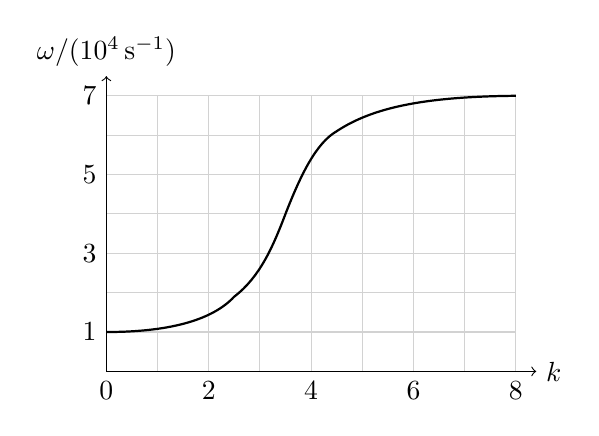
\begin{tikzpicture}[x=.65cm,y=.5cm]
\draw[step=1,gray!35] (0,0) grid (8,7);
\draw[->] (0,0)--(8.4,0) node[right]{$k$};
\draw[->] (0,0)--(0,7.5) node[above]{$\omega/(10^4\,\mathrm{s^{-1}})$};
\foreach \x in {0,2,4,6,8}{\node[below] at (\x,0){$\x$};}
\foreach \y in {1,3,5,7}{\node[left] at (0,\y){$\y$};}
\draw[thick] (0,1) .. controls (1,1) and (2,1.2) .. (2.5,1.9)
 .. controls (3,2.4) and (3.25,3.15) .. (3.5,4)
 .. controls (3.8,5) and (4.1,5.8) .. (4.5,6.1)
 .. controls (5.2,6.7) and (6.2,6.98) .. (8,7);
\end{tikzpicture}\end{center}
\begin{enumerate}[label=\alph*.]
\item 在哪些近似角频率处相速度与群速度相等?
\item 为以最高速度传递脉冲, 应选哪个平均角频率? 该速度多大?
\item 用 $\omega=\omega_0=10^4\,\mathrm{s^{-1}}$ 激励介质会怎样? 提示: 考察 $\omega\to\omega_0$ 时 $v_p,v_g$.
\end{enumerate}
\end{exercise}
\begin{solution}
(a) $v_p=\omega/k$, $v_g=\dd\omega/\dd k$. 两者相等的几何条件是该点的切线穿过坐标原点, 而不是曲线穿过原点. 原图约给两个接点 $k\simeq2.1$ 和 $4.4\,\mathrm{m^{-1}}$, 对应 $\omega\simeq1.5\times10^4$ 和 $6.0\times10^4\,\mathrm{s^{-1}}$. 读图不能给精确等式或过多有效数字.
(b) 窄带脉冲以群速度传播, 选最陡处约 $k=3.5\,\mathrm{m^{-1}}$, $\omega\simeq4\times10^4\,\mathrm{s^{-1}}$. 由附近 $\Delta\omega\simeq(5-3)10^4\,\mathrm{s^{-1}}$, $\Delta k\simeq0.65\,\mathrm{m^{-1}}$, 得最大群速度约 $3\times10^4\,\mathrm{m/s}$. 宽带脉冲会变形, 单一群速度只描述窄带包络.
(c) 当 $\omega\downarrow\omega_0$, $k\to0$, $v_p\to\infty$ 而 $v_g\to0$. 极限是无空间变化的集体振荡, 不能作为向远处运送脉冲能量的行波. 无穷相速度不意味着无穷信号速度. 给定曲线没有提供阻尼或激励耦合, 不能据此断言振幅无限大.
\end{solution}

\begin{exercise}\label{ps:7.3}
原题 Problem 7.3 (30 pts). 无限长弦线密度为 $\rho_L$, 张力为 $T$. 一个高斯脉冲沿弦传播:
$y(x,t)=\exp[-(x-vt)^2/(2\sigma^2)]$.
\begin{enumerate}[label=\alph*.]
\item 计算逆 Fourier 变换, 求组成脉冲的频率分布 $C(\omega)$. 它也是高斯, 宽度记为 $\sigma_\omega$; 可用工具求积分, 但须确定全部常数 (原题指 Georgi 式10.37).
\item 求两高斯宽度之积 $\sigma\sigma_\omega$.
\item 画 $t=0$ 时 $\sigma=1,5$ 的脉冲.
\item 在 $x=0$ 画同样 $\sigma=1,5$ 的 $C(\omega)$; 注意不是令 $\sigma_\omega=1,5$.
\item 比较这两组图形, 描述变化规律.
\end{enumerate}
\end{exercise}
\begin{solution}
(a) 弦速 $v=\sqrt{T/\rho_L}>0$. 明确采用
$y(0,t)=\int_{-\infty}^{\infty}C(\omega)\e^{-\ii\omega t}\dd\omega$,
$C(\omega)=(2\pi)^{-1}\int y(0,t)\e^{\ii\omega t}\dd t$.
令 $\tau=\sigma/v$, 配方或用高斯积分得
\[
C(\omega)=\frac{\tau}{\sqrt{2\pi}}\exp(-\tau^2\omega^2/2)
=\frac{\sigma}{v\sqrt{2\pi}}\exp\left(-\frac{\sigma^2\omega^2}{2v^2}\right).
\]
于是 $y(x,t)=\int C(\omega)\e^{\ii\omega x/v-\ii\omega t}\dd\omega$. 如果将 $1/(2\pi)$ 放在合成式而非分析式, 系数相应乘 $2\pi$; 两种约定不可混用.
(b) 振幅高斯的标准差为 $\sigma_\omega=v/\sigma$, 所以 $\sigma\sigma_\omega=v$ (单位 $\mathrm{m/s}$); 时间宽度与频率宽度之积才为1.
(c)--(e) 下图横轴分别为 $x$ 和 $\omega/v$, 频谱纵轴画 $vC$. 实线 $\sigma=1$, 虚线 $\sigma=5$. 位移峰都为1, 频谱峰分别为 $1/\sqrt{2\pi}$ 和 $5/\sqrt{2\pi}$. 脉冲越宽, 频谱越窄且越高; $\int C\dd\omega=1$ 保持不变.
\begin{center}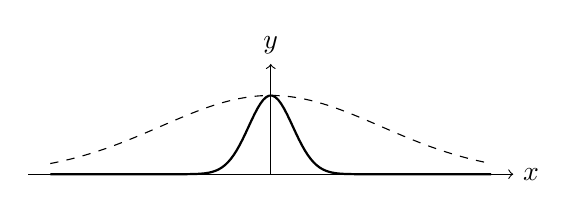
\begin{tikzpicture}[x=.28cm,y=1cm]
\draw[->] (-11,0)--(11,0) node[right]{$x$};\draw[->] (0,0)--(0,1.4) node[above]{$y$};
\draw[thick,domain=-10:10,samples=150] plot (\x,{exp(-\x*\x/2)});
\draw[dashed,domain=-10:10,samples=100] plot (\x,{exp(-\x*\x/50)});
\end{tikzpicture}\quad
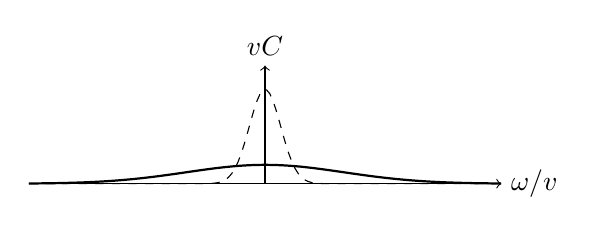
\begin{tikzpicture}[x=1.0cm,y=.6cm]
\draw[->] (-3,0)--(3,0) node[right]{$\omega/v$};\draw[->] (0,0)--(0,2.5) node[above]{$vC$};
\draw[thick,domain=-3:3,samples=100] plot (\x,{exp(-\x*\x/2)/sqrt(2*pi)});
\draw[dashed,domain=-3:3,samples=150] plot (\x,{5*exp(-25*\x*\x/2)/sqrt(2*pi)});
\end{tikzpicture}\end{center}
\end{solution}

\originalsection{作业八}
作业八原件仅有三题, 每题25分, 此处不补造第四题.
\begin{exercise}\label{ps:8.1}
原题 Problem 8.1 (25 pts). 九个质量均为 $m$ 的珠子在边长为 $L$ 的正方形固定框架内, 排成 $3\times3$ 等距格点. 横弦张力为 $T_h$, 竖弦张力为 $T_v$; 不与珠相接的弦端固定, 框架位于 $z=0$. 位移沿 $z$ 方向. 珠坐标是 $(kL/4,jL/4)$, $k,j=1,2,3$; 原图行从下到上为 $j=1,2,3$.
\begin{enumerate}[label=\alph*.]
\item 求简正模及其频率.
\item 令 $T_v=1000T_h$. 按频率递增画九个模, 用 $+,-,0$ 标示珠子的瞬时上下运动或静止. 整体正负可交换. 原图示例最低模全为 $+$; 中间模的三行是 $(-,0,+),(0,0,0),(+,0,-)$.
\end{enumerate}
\end{exercise}
\begin{solution}
(a) 记 $a=L/4$, 位移 $z_{kj}$. 小振幅下张力竖直分量给
\[
m\ddot z_{kj}=\frac{T_h}{a}(z_{k+1,j}+z_{k-1,j}-2z_{kj})+
\frac{T_v}{a}(z_{k,j+1}+z_{k,j-1}-2z_{kj}),
\]
边界指标0和4的位移均为0. 分离变量的九模为
\[
z^{(p,q)}_{kj}(t)=D\sin\frac{p\pi k}{4}\sin\frac{q\pi j}{4}\cos(\omega_{pq}t+\phi),
\quad p,q=1,2,3,
\]
\[
\omega_{pq}^2=\frac4{ma}\left(T_h\sin^2\frac{p\pi}{8}+T_v\sin^2\frac{q\pi}{8}\right),\qquad f_{pq}=\frac{\omega_{pq}}{2\pi}.
\]
代入差分算子即得特征值; 三个一维正弦向量正交且完备, 其张量积覆盖九个自由度.
(b) 一维特征值的三个因子随模指标严格递增. 竖向张力1000倍足以使 $q$ 的变化压过所有 $p$ 的变化, 故顺序依次为 $q=1$ 时的 $(1,1),(2,1),(3,1)$, 然后 $q=2$ 时的 $(1,2),(2,2),(3,2)$, 最后 $q=3$ 时的 $(1,3),(2,3),(3,3)$. 以下每矩阵按上、中、下三行画出, 即 $j=3,2,1$; 零是精确节点.
\[
\begin{array}{c@{\qquad}c@{\qquad}c}
(1,1):\begin{pmatrix}+&+&+\\+&+&+\\+&+&+\end{pmatrix}&
(2,1):\begin{pmatrix}+&0&-\\+&0&-\\+&0&-\end{pmatrix}&
(3,1):\begin{pmatrix}+&-&+\\+&-&+\\+&-&+\end{pmatrix}\\[8pt]
(1,2):\begin{pmatrix}-&-&-\\0&0&0\\+&+&+\end{pmatrix}&
(2,2):\begin{pmatrix}-&0&+\\0&0&0\\+&0&-\end{pmatrix}&
(3,2):\begin{pmatrix}-&+&-\\0&0&0\\+&-&+\end{pmatrix}\\[8pt]
(1,3):\begin{pmatrix}+&+&+\\-&-&-\\+&+&+\end{pmatrix}&
(2,3):\begin{pmatrix}+&0&-\\-&0&+\\+&0&-\end{pmatrix}&
(3,3):\begin{pmatrix}+&-&+\\-&+&-\\+&-&+\end{pmatrix}
\end{array}
\]
\end{solution}

\begin{exercise}\label{ps:8.2}
原题 Problem 8.2 (25 pts). 光从真空 $n_1=1$ 入射透明平板 $n_2$, 然后进入介质 $n_3$. 两界面平行. 入射角 $\alpha=60^\circ$, 最后出射角 $\beta=30^\circ$, 两角都从法线量起. 原图在板内光线更接近法线, 不给板内角数值.
\begin{enumerate}[label=\alph*.]
\item $n_2$ 可能取哪些值?
\item 求 $n_3$.
\end{enumerate}
\end{exercise}
\begin{solution}
令板内折射角为 $r$. 平行界面两次 Snell 定律给
$n_1\sin\alpha=n_2\sin r=n_3\sin\beta=\sqrt3/2$.
(a) 存在穿过有限厚度平板的实射线要求 $\sin r<1$, 故 $n_2>\sqrt3/2$. $n_2=\sqrt3/2$ 是沿界面的掠射极限, 并不能穿越板厚. 若只要求实折射角而不要求穿板, 可写非严格下界. 原题未显式要求普通 $n\ge1$ 介质; 若再把原图的板内角比入射角小作为定性条件, 则需 $n_2>1$. 若进一步把示意图板内射线比末层射线更靠近法线视为附加条件, 即 $r<\beta$, 则要求 $n_2>n_3=\sqrt3$; 题中文字角度本身没有提供这一额外约束.
(b) $n_3=\sin60^\circ/\sin30^\circ=\sqrt3\simeq1.732$, 与中间层折射率无关. 这是平行界面中切向波数守恒的结果.
\end{solution}

\begin{exercise}\label{ps:8.3}
原题 Problem 8.3 (25 pts). 近水平阳光进入暗云中的水滴, 经一次内反射后射出, 形成约 $40^\circ$--$42^\circ$ 的彩虹. 入射角 $\theta$ 从水滴表面法线量起, $\alpha$ 是出射反向光线与入射光线正向延长线的夹角, 即相对反太阳方向的彩虹角.
\begin{enumerate}[label=\alph*.]
\item 求 $\alpha(\theta,n)$, 其中 $n$ 是水的折射率. 对 $0\le\theta\le90^\circ$ 作图并求最大值; 取 $n=1.33$, 可用任意绘图工具.
\item 为什么彩虹出现在该极值角?
\item 仰望彩虹时哪种颜色位于更高角度? 提示: 红光折射率略小于蓝光.
\item 定性解释双彩虹. 第二道彩虹哪种颜色更高?
\end{enumerate}
\end{exercise}
\begin{solution}
(a) 折射角 $r=\arcsin(\sin\theta/n)$. 两次折射的总偏转为 $2(\theta-r)$, 一次反射偏转 $\pi-2r$, 总偏向角 $D=\pi+2\theta-4r$. 因而
\[
\alpha=\pi-D=4r-2\theta.
\]
导数为 $\alpha'=4\cos\theta/(n\cos r)-2$. 极值满足 $2\cos\theta=n\cos r$, 结合 Snell 定律得
\[
\sin^2\theta_*=(4-n^2)/3.
\]
$n=1.33$ 时 $\theta_*\simeq59.5849^\circ$, $r_*\simeq40.4216^\circ$, $\alpha_{\max}\simeq42.5164^\circ$. 端点 $\alpha(0)=0$, $\alpha(90^\circ)\simeq15.0^\circ$, 极值确为最大. 下图直接用已推导函数绘制, 不充当证明.
\begin{center}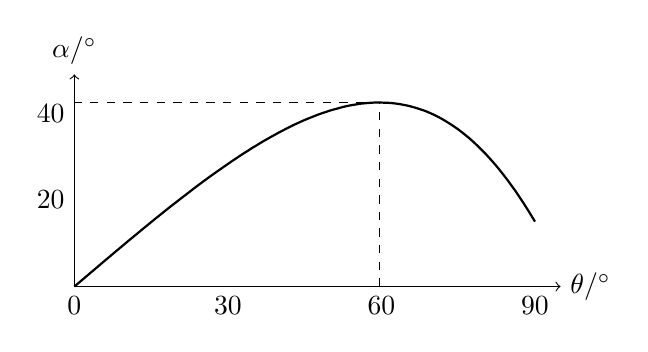
\begin{tikzpicture}[x=.065cm,y=.055cm]
\draw[->] (0,0)--(95,0) node[right]{$\theta/{}^\circ$};
\draw[->] (0,0)--(0,49) node[above]{$\alpha/{}^\circ$};
\foreach \x in {0,30,60,90}{\node[below] at (\x,0){$\x$};}
\foreach \y in {20,40}{\node[left] at (0,\y){$\y$};}
\draw[thick,domain=0:90,samples=120] plot (\x,{4*asin(sin(\x)/1.33)-2*\x});
\draw[dashed] (59.585,0)--(59.585,42.516)--(0,42.516);
\end{tikzpicture}\end{center}
(b) 在 $\alpha'=0$ 附近, 一段较宽的入射角区间挤到狭小的出射角区间, 形成射线密度增强的焦散. 光源有限角宽、波动衍射与水滴大小使实际亮峰有限.
(c) 固定 $\theta$, 较小 $n$ 给较大 $r$, 因而较大 $\alpha$; 极值也如此. 主虹红色在外侧, 仰望上方弧时红色更高.
(d) 两次内反射给第二道虹. 总偏转为 $D_2=2\pi+2\theta-6r$, 所见角为 $\alpha_2=D_2-\pi=\pi+2\theta-6r$, 极值是最小值, 通常约 $51^\circ$. 较大折射率使 $r$ 更小而 $\alpha_2$ 更大, 所以副虹蓝紫在外侧且更高, 颜色次序相反; 多一次反射也使其较暗.
\end{solution}

\originalsection{作业九}
\begin{exercise}\label{ps:9.1}
原题 Problem 9.1 (20 pts). 把电离层视为折射率 $n=\sqrt{1-\omega_p^2/\omega^2}$ 的介质, $\omega_p$ 为常数等离子体角频率.
\begin{enumerate}[label=\alph*.]
\item 画电磁波传播波矢的大小 $k$ 随 $\omega$ 的曲线.
\item 当 $\omega=\sqrt2\omega_p$ 时求相速度和群速度.
\item $\omega<\omega_p$ 时电离层内的电磁扰动会怎样?
\end{enumerate}
\end{exercise}
\begin{solution}
(a) 在传播区 $\omega\ge\omega_p$,
$k=\sqrt{\omega^2-\omega_p^2}/c$, 即 $\omega^2=\omega_p^2+c^2k^2$. 曲线从 $(\omega_p,0)$ 出发, 斜率先趋于无穷, 然后接近直线 $k=\omega/c$. 无量纲图如下.
\begin{center}\begin{tikzpicture}[x=1.2cm,y=1cm]
\draw[->] (0,0)--(4.4,0) node[right]{$\omega/\omega_p$};\draw[->] (0,0)--(0,4.3) node[above]{$ck/\omega_p$};
\draw[dashed] (0,0)--(4,4);\draw[thick,domain=1:4,samples=120] plot (\x,{sqrt(\x*\x-1)});
\node[below] at (1,0){$1$};
\end{tikzpicture}\end{center}
(b) $v_p=\omega/k=c/\sqrt{1-\omega_p^2/\omega^2}$, $v_g=c\sqrt{1-\omega_p^2/\omega^2}$, 故 $v_p=\sqrt2c$, $v_g=c/\sqrt2$. $v_pv_g=c^2$, 超光速相速度不表示超光速能量传播.
(c) $k=\ii\kappa$, $\kappa=\sqrt{\omega_p^2-\omega^2}/c$, 界面激励产生随深度衰减的倏逝场 $\e^{-\kappa x}$. 无耗散半无限介质不能支持该频率的体内传播模式, 入射能量主要被反射. 有限厚层可有隧穿; 不能把虚波数的模 $\kappa$ 误画成实传播波数.
\end{solution}

\begin{exercise}\label{ps:9.2}
原题 Problem 9.2 (20 pts). 光沿 $+z$ 传播, 入射为沿 $y$ 的线偏振, 强度 $I_0$. 先后放置理想偏振片 A,B, 其透光轴相对 $y$ 的角为 $\theta_A,\theta_B$. 每片全透过沿轴分量、完全阻挡垂直分量, $I\propto\langle E^2\rangle$.
\begin{enumerate}[label=\alph*.]
\item 求 A 后强度 $I_a$.
\item 求 A 和 B 后强度 $I_b$.
\end{enumerate}
现以四分之一波片 C 替换 A. C 只有相位作用, 其快轴与 $y$ 的夹角为 $\theta_C$, 慢轴正交于快轴; 慢轴分量相对快轴延迟 $\pi/2$.
\begin{enumerate}[label=\alph*.,start=4]
\item 求 C 后强度 $I_c$.
\item 令 B 的轴沿 $y$ ($\theta_B=0$), 求通过 C,B 后强度 $I_b(\theta_C)$.
\end{enumerate}
原件的小问编号为 a,b,d,e, 没有 c, 此处照原编号保留.
\end{exercise}
\begin{solution}
(a) Malus 定律给 $I_a=I_0\cos^2\theta_A$.
(b) A 后偏振方向沿 A 轴, 故 $I_b=I_0\cos^2\theta_A\cos^2(\theta_B-\theta_A)$.
(d) 波片不吸收能量, 两个正交分量强度相加, $I_c=I_0(\cos^2\theta_C+\sin^2\theta_C)=I_0$.
(e) 记快轴 $\mathbf f=\sin\theta_C\hat{\mathbf x}+\cos\theta_C\hat{\mathbf y}$, 慢轴 $\mathbf s=\cos\theta_C\hat{\mathbf x}-\sin\theta_C\hat{\mathbf y}$. 则入射 Jones 向量在这组基中是 $E_0(\cos\theta_C,-\sin\theta_C)$. 慢轴乘相位因子 $\ii$ (改变时间约定则用 $-\ii$, 强度不变). 出射 $y$ 振幅为 $E_0(\cos^2\theta_C+\ii\sin^2\theta_C)$, 所以
\[
I_b=I_0(\cos^4\theta_C+\sin^4\theta_C)
=I_0\left(1-\frac12\sin^2 2\theta_C\right).
\]
快轴沿 $y$ 时仍为线偏振, 全透过; $\theta_C=45^\circ$ 时成为圆偏振, B 透过一半.
\end{solution}

\begin{exercise}\label{ps:9.3}
原题 Problem 9.3 (20 pts). 单色平面电磁波在介质中沿 $+z$ 传播, 电场线偏振方向与 $x$ 轴夹 $30^\circ$. 角频率为 $\omega$, 介质相对介电常数为 $\kappa_e$.
\begin{enumerate}[label=\alph*.]
\item 用 $\omega,c,\kappa_e,E_0$ 写 $E_x,E_y,B_x,B_y$, 其中 $E_0$ 是电场振幅.
\item 求穿过垂直传播方向表面的单位面积能量传输率.
\item 写介质内电磁波动方程.
\end{enumerate}
\end{exercise}
\begin{solution}
采用题目通常隐含的均匀、无损、非磁介质模型 $\epsilon=\kappa_e\epsilon_0$, $\mu=\mu_0$, 且在该频率附近忽略色散. 于是 $n=\sqrt{\kappa_e}$, $v=c/n$, $k=n\omega/c$. 相位 $\Phi=kz-\omega t$ 可加任意常数.
(a)
\[
\begin{aligned}
E_x&=\tfrac{\sqrt3}{2}E_0\cos\Phi,&E_y&=\tfrac12 E_0\cos\Phi,\\
B_x&=-\tfrac{n}{2c}E_0\cos\Phi,&B_y&=\tfrac{\sqrt3n}{2c}E_0\cos\Phi.
\end{aligned}
\]
因为 $\mathbf B=(1/v)\hat{\mathbf z}\times\mathbf E$; $E_z=B_z=0$.
(b) 瞬时 Poynting 向量为 $\mathbf S=(nE_0^2/\mu_0c)\cos^2\Phi\,\hat{\mathbf z}$, 周期平均输运率
$I=nE_0^2/(2\mu_0c)=\tfrac12\epsilon_0cnE_0^2$.
(c) $\nabla^2\mathbf E=(\kappa_e/c^2)\mathbf E_{tt}$, $\nabla^2\mathbf B=(\kappa_e/c^2)\mathbf B_{tt}$. 对沿 $z$ 的波可将 $\nabla^2$ 换成 $\partial_z^2$. 若介质磁性或色散不可忽略, 仅给 $\kappa_e$ 不足以确定全部传播与能量性质.
\end{solution}

\begin{exercise}\label{ps:9.4}
原题 Problem 9.4 (20 pts). 一个非相对论电子在磁场中作螺旋运动,
$\mathbf r(t)=\alpha\hat{\mathbf x}\cos\beta t+\alpha\hat{\mathbf y}\sin\beta t+\gamma t\hat{\mathbf z}$.
\begin{enumerate}[label=\alph*.]
\item 远处天文学家位于 (i) $(0,0,R)$, (ii) $(R/\sqrt2,0,R/\sqrt2)$, (iii) $(R,0,0)$, $R\gg\alpha$. 分别给观测辐射频率 $\nu$、波矢和偏振状态.
\item 写位于 $B=(0,0,R)$ 的辐射电、磁场完整表达式.
\item 用 Larmor 公式 $P=q^2|\mathbf a|^2/(6\pi\epsilon_0c^3)$ 求每秒总辐射能量.
\item 以源为中心、半径 $R$ 的球面上, 周期平均 Poynting 向量的最大和最小值之比为多少?
\end{enumerate}
\end{exercise}
\begin{solution}
以下按非相对论远区辐射的最低阶计算: $\alpha\beta/c\ll1$, $|\gamma|/c\ll1$, 且观测期间源的漂移远小于 $R$. $R\gg\alpha$ 本身并不保证任意长时间仍满足远区定距近似. 取电子电荷 $q=-e$, $e>0$, 迟滞时间 $t_r=t-R/c$,
\[
\mathbf a=-\alpha\beta^2(\hat{\mathbf x}\cos\beta t_r+\hat{\mathbf y}\sin\beta t_r),\quad
\mathbf E_{\rm rad}=\frac{q}{4\pi\epsilon_0c^2R}\hat{\mathbf n}\times(\hat{\mathbf n}\times\mathbf a),\quad
\mathbf B_{\rm rad}=\frac1c\hat{\mathbf n}\times\mathbf E_{\rm rad}.
\]
匀速 $z$ 分量没有加速度, 不产生最低阶辐射. 定义 $K=q\alpha\beta^2/(4\pi\epsilon_0c^2R)$.
(a) 最低阶三个方向的频率均为 $\nu=\beta/(2\pi)$, 波矢为 $\mathbf k=(\beta/c)\hat{\mathbf n}$.
(i) $\mathbf E=K(\hat{\mathbf x}\cos\beta t_r+\hat{\mathbf y}\sin\beta t_r)$, 是圆偏振. (ii) $\hat{\mathbf n}=(\hat{\mathbf x}+\hat{\mathbf z})/\sqrt2$, 在横向基 $\mathbf e_1=(\hat{\mathbf x}-\hat{\mathbf z})/\sqrt2$, $\mathbf e_2=\hat{\mathbf y}$ 中,
$\mathbf E=K[(\mathbf e_1/\sqrt2)\cos\beta t_r+\mathbf e_2\sin\beta t_r]$, 是轴比 $1:\sqrt2$ 的椭圆偏振. (iii) $\mathbf E=K\hat{\mathbf y}\sin\beta t_r$, 是沿 $y$ 的线偏振. 电场矢量表达式明确了旋转方向, 避免圆偏振左右手命名约定的歧义.
(b) 在 B 点,
\[
\mathbf E_B=K[\hat{\mathbf x}\cos\beta(t-R/c)+\hat{\mathbf y}\sin\beta(t-R/c)],
\]
\[
\mathbf B_B=\frac Kc[-\hat{\mathbf x}\sin\beta(t-R/c)+\hat{\mathbf y}\cos\beta(t-R/c)].
\]
这是完整的 $1/R$ 辐射项, 不包括 $1/R^2$ 的近场或静电场. 若保留漂移引起的一阶 Doppler 修正, 迟滞条件给 $t_r\simeq(t-R/c)/(1-\gamma n_z/c)$, 三方向的观测角频率相应为 $\beta/(1-\gamma n_z/c)$. 要同阶精确计算场幅与角分布, 还须保留移动电荷辐射场的速度因子, 不能只替换频率而称为完整相对论场.
(c) $|\mathbf a|=\alpha\beta^2$, 故 $P=e^2\alpha^2\beta^4/(6\pi\epsilon_0c^3)$.
(d) 令 $\vartheta$ 是观测方向与 $z$ 轴的夹角. 横向加速度平方平均为
$\langle|\mathbf a_\perp|^2\rangle=\alpha^2\beta^4(1+\cos^2\vartheta)/2$. 因而
\[
\langle S_r\rangle=\frac{e^2\alpha^2\beta^4}{32\pi^2\epsilon_0c^3R^2}(1+\cos^2\vartheta).
\]
两极最大、赤道最小, 比值为2. 对球面积分用 $\int(1+\cos^2\vartheta)\dd\Omega=16\pi/3$, 恰好复得 Larmor 总功率.
\end{solution}

\begin{exercise}\label{ps:9.5}
原题 Problem 9.5 (20 pts). 光从空气射向玻璃平面界面, 入射电场有平行入射面的 $\mathbf E_\parallel$ 和垂直入射面的 $\mathbf E_\perp$ 两分量. 原图空气在上、玻璃在下, 入射与反射在上半空间; 入射角为 Brewster 角 $\theta_B$.
\begin{enumerate}[label=\alph*.]
\item 像原入射线图那样用图示标出反射和折射线中的偏振分量.
\item 用 Snell 定律给 Brewster 角的定义方程.
\item 用玻璃中电荷的加速度解释反射光偏振方向, 为什么反射光电场平行于界面?
\end{enumerate}
\end{exercise}
\begin{solution}
(a) 反射 $p$ 分量为零, 只剩 $s$ 分量, 即垂直入射面而平行界面. 折射光一般同时有 $p,s$ 分量. 示意图纸面是入射面, $\odot$ 表示出纸面的 $s$ 偏振, 短线表示纸面内且垂直光线的 $p$ 分量.
\begin{center}\begin{tikzpicture}[scale=.85]
\draw[thick] (-3,0)--(3,0);\draw[dashed] (0,-2.2)--(0,2.2);
\draw[->] (-2,1.5)--(0,0);\draw[->] (0,0)--(2,1.5);
\draw[->] (0,0)--(1.3,-1.73);
\node at (-1.4,1.4){$\odot$};\draw (-1.7,.75)--(-1.1,1.55);
\node at (1.45,1.4){$\odot$};\node[right] at (2,1.5){仅 $s$};
\node at (.9,-1.35){$\odot$};\draw (.5,-1.45)--(1.3,-.85);
\node[left] at (-2.2,.2){空气};\node[left] at (-2.2,-.4){玻璃};
\end{tikzpicture}\end{center}
(b) 反射与折射方向互相垂直, $\theta_B+\theta_t=\pi/2$, 而 $n_a\sin\theta_B=n_g\sin\theta_t=n_g\cos\theta_B$, 故 $\tan\theta_B=n_g/n_a=n_g$.
(c) 折射电场驱动玻璃中的电荷振荡. $p$ 偏振振荡方向处于入射面、垂直折射线. 在 Brewster 几何中该方向正好沿反射线; 偶极辐射沿加速度方向为零, 因此无反射 $p$ 波. $s$ 振荡垂直入射面, 在反射方向可以辐射, 所以仅保留与界面平行的 $s$ 偏振. 这不是说所有角度的反射光都只有该偏振.
\end{solution}

\originalsection{作业十}
\begin{exercise}\label{ps:10.1}
原题 Problem 10.1 (20 pts). 频率 $\nu$ 的点光源 S 在空气 ($n=1$) 中, 距理想导体平面 $L$. 观察者距 S 很远, 位于垂直镜面的方向, 与 S 同在导体外侧. 忽略 S 对反射光的吸收.
\begin{enumerate}[label=\alph*.]
\item 哪些 $L$ 使观察者见干涉极大?
\item 哪些 $L$ 使观察者见干涉极小?
\item 在源与镜之间放折射率为 $n$ 的玻璃, 对给定 $L$ 要使极大与极小交换, 最小厚度多大? 假设玻璃表面无反射.
\end{enumerate}
\end{exercise}
\begin{solution}
令 $\lambda=c/\nu$. 镜面理想导体的切向电场反射系数为 $-1$, 引入 $\pi$ 相变. 直接光与反射光程差为 $2L$, 总相位差 $\delta=4\pi L/\lambda+\pi$.
(a) 极大 $\delta=2\pi m$, 所以 $L=(2j+1)\lambda/4$, $j=0,1,\ldots$.
(b) 极小 $\delta=(2m+1)\pi$, 所以 $L=j\lambda/2$. 对源实际在镜外须 $j\ge1$; $j=0$ 是形式边界极限. 远处两光振幅可近似相等, 此时极小为零.
(c) 玻璃替代厚度 $d$ 的空气, 反射光往返玻璃, 增加光程 $2(n-1)d$. 交换极值所需最小正相差为 $\pi$, 故 $d_{\min}=\lambda/[4(n-1)]$ ($n>1$). 若此厚度超过可用间隙 $L$, 不能在题设位置完整放入这种平板.
\end{solution}

\begin{exercise}\label{ps:10.2}
原题 Problem 10.2 (20 pts). 三条长窄狭缝依次沿竖直方向等距排列, 相邻中心距 $d=1\,\mathrm{mm}$. 单色波长 $\lambda=500\,\mathrm{nm}$, 屏距 $L=5\,\mathrm m$. 单缝足够窄, 忽略单缝衍射. 各未遮挡单缝在屏上的强度为 $I_0$. 屏中心坐标 $x=0$.
\begin{enumerate}[label=\alph*.]
\item 先完全挡住最上缝, 求中心极大到第一极小的距离, 单位毫米.
\item 画中心和左右各两个极大共五个峰的强度曲线, 标轴并给五峰强度.
\item 打开最上缝, 再求中心到第一极小的距离.
\item 画打开三缝后的五个相邻极大及标轴.
\item 给这五个峰各自强度.
\item 最上缝改用只透过一半入射强度、但不改变相位或偏振的材料遮盖. 最大峰强度是多少? 五个相邻峰中哪些达到它?
\item 写以 $x$ 为未知数、能求中心最近强度极小的方程, 不必求解.
\item 画此时的五峰强度曲线.
\end{enumerate}
\end{exercise}
\begin{solution}
采用小角远场 $\delta=2\pi dx/(\lambda L)$, 记 $X=\lambda L/d=2.5\,\mathrm{mm}$, $u=x/X$.
(a),(b) 两缝复振幅 $1+\e^{\ii\delta}$, $I/I_0=4\cos^2(\pi u)$. 第一极小 $x=X/2=1.25\,\mathrm{mm}$, 五极大位于 $x=-2X,-X,0,X,2X$, 强度均 $4I_0$.
(c)--(e) 三缝复振幅 $1+\e^{\ii\delta}+\e^{2\ii\delta}$, 因而
$I/I_0=(1+2\cos\delta)^2$. 最近零点 $\delta=2\pi/3$, 即 $x=X/3=0.8333\,\mathrm{mm}$. 中心附近五个\textbf{相邻局部极大}在 $x=-X,-X/2,0,X/2,X$, 强度依次 $9I_0,I_0,9I_0,I_0,9I_0$. 三缝有次极大, 不能把五个相邻峰都当作主极大. 若题意只数主峰, $x=-2X,-X,0,X,2X$ 的五个主峰都为 $9I_0$, 中间仍须画出次峰.
(f)--(h) 半强度透过率给\textbf{振幅}比 $a=1/\sqrt2$, 并非 $1/2$. 取最上缝为第三项, 振幅
$F=1+\e^{\ii\delta}+a\e^{2\ii\delta}$,
\[
\frac{I}{I_0}=2+a^2+2(1+a)\cos\delta+2a\cos2\delta.
\]
最大值在 $\delta=2\pi m$, $I_{\max}=(2+a)^2I_0=(9/2+2\sqrt2)I_0\simeq7.3284I_0$. 五相邻峰中中心及左右 $x=\pm X$ 主峰达到此值; $x=\pm X/2$ 的次峰为 $a^2I_0=I_0/2$.
(g) 对 $x$ 求导,
\[
\sin\left(\frac{2\pi x}{X}\right)
\left[1+a+4a\cos\left(\frac{2\pi x}{X}\right)\right]=0.
\]
最近非零极小应选第二因子为零且 $0<x<X/2$, 排除中心与次峰对应的第一因子零点. 最近极小不再为零, 因为三个不等振幅不能在该相位完全抵消.
下面三图按上述解析式绘出, 横轴 $u=x/X$, 纵轴 $I/I_0$. 第一幅涵盖五个两缝峰; 后两幅涵盖五个相邻三缝峰.
\begin{center}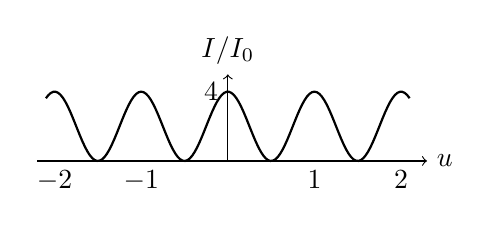
\begin{tikzpicture}[x=1.1cm,y=.22cm]
\draw[->] (-2.2,0)--(2.3,0) node[right]{$u$};\draw[->] (0,0)--(0,5) node[above]{$I/I_0$};
\draw[thick,domain=-2.1:2.1,samples=150] plot (\x,{4*cos(180*\x)^2});
\foreach \x in {-2,-1,1,2}{\node[below] at (\x,0){$\x$};}\node[left] at (0,4){$4$};
\end{tikzpicture}\par
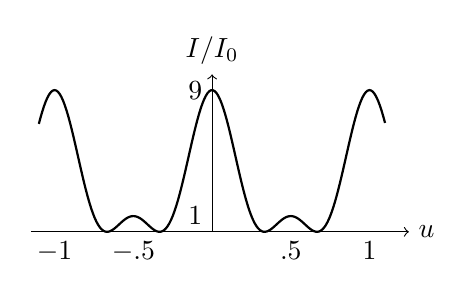
\begin{tikzpicture}[x=2cm,y=.2cm]
\draw[->] (-1.15,0)--(1.25,0) node[right]{$u$};\draw[->] (0,0)--(0,10) node[above]{$I/I_0$};
\draw[thick,domain=-1.1:1.1,samples=200] plot (\x,{(1+2*cos(360*\x))^2});
\foreach \x in {-1,-.5,.5,1}{\node[below] at (\x,0){$\x$};}\node[left] at (0,9){$9$};\node[left] at (0,1){$1$};
\end{tikzpicture}\par
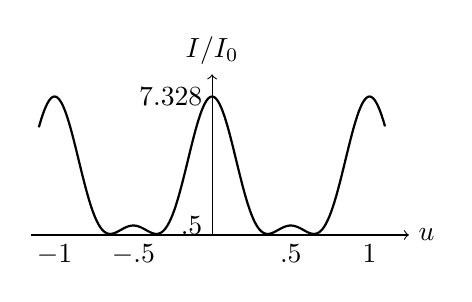
\begin{tikzpicture}[x=2cm,y=.24cm]
\draw[->] (-1.15,0)--(1.25,0) node[right]{$u$};\draw[->] (0,0)--(0,8.5) node[above]{$I/I_0$};
\draw[thick,domain=-1.1:1.1,samples=200] plot (\x,{2.5+2*(1+1/sqrt(2))*cos(360*\x)+sqrt(2)*cos(720*\x)});
\foreach \x in {-1,-.5,.5,1}{\node[below] at (\x,0){$\x$};}\node[left] at (0,7.328){$7.328$};\node[left] at (0,.5){$.5$};
\end{tikzpicture}\end{center}
\end{solution}

\begin{exercise}\label{ps:10.3}
原题 Problem 10.3 (20 pts). 两个沿 $z$ 的偶极辐射源沿 $x$ 轴相距 $\lambda/2$, 观察距离 $r\gg\lambda$. 原图的 $\theta$ 在 $x$--$y$ 平面\textbf{从正 $y$ 轴朝正 $x$ 轴量起}, 故 $\hat{\mathbf n}=(\sin\theta,\cos\theta,0)$.
\begin{enumerate}[label=\alph*.]
\item 两源同相时, 求 $\theta=0,\pi/3,\pi/2,\pi$ 的相对辐射强度.
\item 两源相差 $\pi$ 时重复上一问.
\item 改为相距 $\lambda/4$、相差 $\pi/2$, 求 $\theta=0,\pi/2,3\pi/2$ 的相对强度.
\end{enumerate}
\end{exercise}
\begin{solution}
令两源位于 $x=0,d$, 等振幅; 第二源复振幅相对第一源相位为 $\phi$. 以时间约定 $\e^{-\ii\omega t}$, 远区总复振幅比例为 $1+\e^{\ii(\phi-kd\sin\theta)}$. 在 $x$--$y$ 平面, 单个 $z$ 偶极的方向因子相同, 记其强度为 $I_1$, 则
\[
I/I_1=2+2\cos(\phi-kd\sin\theta).
\]
(a) $kd=\pi$, $\phi=0$, 强度依次为
$4$, $2+2\cos(\sqrt3\pi/2)\simeq0.17455$, $0$, $4$.
(b) $\phi=\pi$, 依次为 $0$, $2-2\cos(\sqrt3\pi/2)\simeq3.82545$, $4$, $0$.
(c) $kd=\pi/2$, 取第二源相位 $\phi=+\pi/2$, 则三个方向为 $2,4,0$. 若第二源的相位是 $-\pi/2$, 则为 $2,0,4$. 原文只说两源相差 $\pi/2$, 未标注哪一源超前, 因此应说明该方向选择. 若用全相干最大强度 $4I_1$ 归一, 将各数除以4即可.
\end{solution}

\begin{exercise}\label{ps:10.4}
原题 Problem 10.4 (20 pts). 少量油 ($n_o=1.45$) 在湖面 ($n_w=1.33$) 上扩散, 膜厚连续减小. 观察近垂直入射的白色天空光反射. 原表波长: 蓝 $480\,\mathrm{nm}$, 绿 $530\,\mathrm{nm}$, 红 $650\,\mathrm{nm}$; 白包含所有可见波长, 黑表示无可见光.
\begin{enumerate}[label=\alph*.]
\item 初始厚膜肉眼为白色. 用红色窄带滤镜观察, 强度从亮出发, 经10次极小后重新到极大. 膜厚改变多少?
\item 膜足够薄才肉眼呈色. 在什么干涉级次 $m$, 红色相长厚度开始超过蓝色\textbf{下一个更高阶}的相长厚度? 更厚时可见光不同部分会重叠.
\item 平湖面油膜刚呈绿色时, 风生表面波经过使颜色随时间变化. 颜色朝光谱哪一端改变? 提示: 膜内光程差正比于光线与法线夹角的余弦.
\end{enumerate}
\end{exercise}
\begin{solution}
空气到油的反射有 $\pi$ 相变, 油到水的反射无相变. 因此近正入射反射相长条件是
$2n_ot=(m+1/2)\lambda$, $m=0,1,2,\ldots$; 相消为 $2n_ot=m\lambda$. 两反射振幅不相等, 实际极小未必完全黑.
(a) 相邻红色极大厚度差为 $\lambda_R/(2n_o)$. 经过10个极小即经过10个完整极大间隔, 厚度减少
$\Delta t=10\lambda_R/(2n_o)=2241.38\,\mathrm{nm}\simeq2.24\,\mu\mathrm m$.
(b) 用本解答的零起始级次, 条件为
$(m+1/2)650>(m+3/2)480$, 即 $170m>395$, 所以首次为 $m=3$.
对应红厚度 $t_R=3.5(650)/(2\times1.45)=784.48\,\mathrm{nm}$, 下一个蓝阶厚度 $t_B=4.5(480)/(2\times1.45)=744.83\,\mathrm{nm}$. 若用 $2n_ot=(m-1/2)\lambda$, $m=1,2,\ldots$, 同一物理阶次标为 $m=4$. 若用奇数半波级次 $2n_ot=m\lambda/2$, 则标为 $m=7$; 必须先给级次约定再报数.
(c) 若膜厚在局部波面上不变, 倾斜使膜内角 $r$ 增大, 相长波长
$\lambda_m=2n_ot\cos r/(m+1/2)$ 减小, 颜色由绿向蓝紫端移. 坡度周期变化则往复变化. 若水波还改变膜厚, 其效应需另行给定, 不能只由角度提示推出.
\end{solution}

\begin{exercise}\label{ps:10.5}
原件印作 Problem 5 (20 pts), 此处对应作业十第5题, 保留其原印编号. 两条平行长缝宽均为 $a$, 中心间距为 $b$, 由波长 $\lambda$ 的平行光照射. 远处屏上强度按 $s=\sin\psi$ 作图. 原图横轴范围 $-0.8$ 到 $0.8$, 中心峰约为4, 干涉零点约在 $s=\pm0.10,\pm0.30,\pm0.50,\pm0.70$, 包络首零约在 $s=\pm1/3$. 下图据该图的零点结构重绘, 不给定绝对光强.
\begin{center}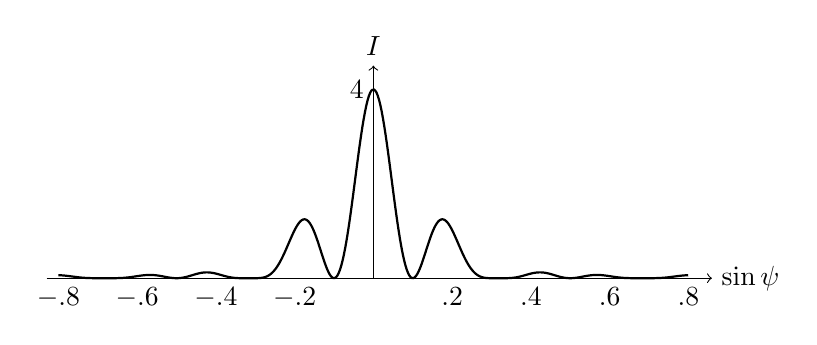
\begin{tikzpicture}[x=5cm,y=.6cm]
\draw[->] (-.83,0)--(.86,0) node[right]{$\sin\psi$};\draw[->] (0,0)--(0,4.5) node[above]{$I$};
\foreach \x in {-.8,-.6,-.4,-.2,.2,.4,.6,.8}{\node[below] at (\x,0){$\x$};}
\node[left] at (0,4){$4$};
\draw[thick,domain=-.8:-.001,samples=240] plot (\x,{4*(sin(540*\x)/(3*pi*\x))^2*cos(900*\x)^2});
\draw[thick,domain=.001:.8,samples=240] plot (\x,{4*(sin(540*\x)/(3*pi*\x))^2*cos(900*\x)^2});
\end{tikzpicture}\end{center}
\begin{enumerate}[label=\alph*.]
\item 由图估计 $a/\lambda,b/\lambda$.
\item 将中心间距加倍为 $2b$, 保持缝宽 $a$ 不变. 画 $I$ 对 $\sin\psi$ 的曲线, 横轴保持原尺度并标注; 纵轴可任意归一. 原题的 ``widened'' 按后续明确条件理解为两缝间距增大, 而非缝宽变大.
\end{enumerate}
\end{exercise}
\begin{solution}
(a) Fraunhofer 双缝公式是
\[
I(s)=4I_0\left[\frac{\sin(\pi as/\lambda)}{\pi as/\lambda}\right]^2
\cos^2(\pi bs/\lambda).
\]
包络首零 $a|s|/\lambda=1$, 读图 $|s|\simeq1/3$ 给 $a\simeq3\lambda$. 干涉最近零 $|s|=\lambda/(2b)\simeq0.10$, 给 $b\simeq5\lambda$. 旁峰位置受包络影响, 不宜把其位置当成精确干涉主极大. 此估计还可用原图相邻干涉零点间距约0.20交叉检查.
(b) 新曲线
\[
I_{\rm new}(s)=4I_0\left[\frac{\sin(3\pi s)}{3\pi s}\right]^2\cos^2(10\pi s).
\]
包络不变, 干涉周期减半, 零点为 $s=(2j+1)/20$, 主干涉极大候选为 $s=j/10$, 但实际局部峰因包络而略偏移. 下图横轴与题面相同, 纵轴仍以 $I_0$ 归一, $s=0$ 取连续极限4.
\begin{center}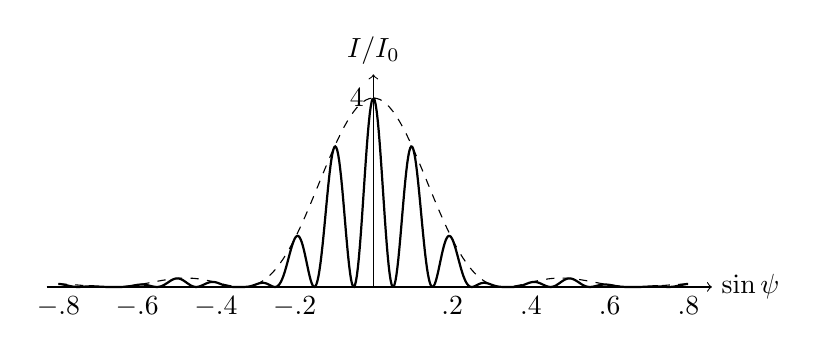
\begin{tikzpicture}[x=5cm,y=.6cm]
\draw[->] (-.83,0)--(.86,0) node[right]{$\sin\psi$};\draw[->] (0,0)--(0,4.5) node[above]{$I/I_0$};
\foreach \x in {-.8,-.6,-.4,-.2,.2,.4,.6,.8}{\node[below] at (\x,0){$\x$};}\node[left] at (0,4){$4$};
\draw[dashed,domain=-.8:-.001,samples=100] plot (\x,{4*(sin(540*\x)/(3*pi*\x))^2});
\draw[dashed,domain=.001:.8,samples=100] plot (\x,{4*(sin(540*\x)/(3*pi*\x))^2});
\draw[thick,domain=-.8:-.001,samples=320] plot (\x,{4*(sin(540*\x)/(3*pi*\x))^2*cos(1800*\x)^2});
\draw[thick,domain=.001:.8,samples=320] plot (\x,{4*(sin(540*\x)/(3*pi*\x))^2*cos(1800*\x)^2});
\end{tikzpicture}\end{center}
\end{solution}
